\chapter{Suavizado}

\hline
\linebreak 

Existen unos tipos de operaciones sobre im�genes como el suavizado y la extracci�n de bordes que reciben el nombre de transformaciones de vecindad.

\section{Vecindad}
Se dice que todo p�xel p, de coordenadas (x, y) tiene 4 p�xeles que establecen con �l una relaci�n de vecindad horizontal y vertical que son:

\begin{center}
Horizontal: (x - 1, y),  (x + 1, y) 	
Vertical:  (x, y - 1),  (x, y + 1)
\end{center} 

Estos cuatro p�xeles definen lo que se conoce como entorno de vecindad-4.
Por tanto vecinos de un p�xel (p) de coordenadas (x, y): (excepto bordes)
\begin{itemize}
\item N_{4}(p) = 4-vecinos de p	{(x-1,y),(x+1,y),(x,y-1),(x,y+1)}
\item N_{d}(p) = vecinos diagonales de p {(x+1,y+1),(x-1,y+1),(x+1,y-1),(x-1,y-1)}
\item N_{8}(p) = 8-vecinos de p	N_{4}(p) \cup N_{d}(4)
\end{itemize} 

\begin{center}
\begin{tabular}{|c|c|c|}
\hline (x-1, y-1) & (x, y-1) & (x+1, y-1) \\ 
\hline (x-1, y) & (x, y) & (x+1, y) \\ 
\hline (x-1, y+1) & (x, y+1) & (x+1, y+1) \\ 
\hline 
Entorno de vecindad del p�xel (x, y)
\end{tabular} 
\end{center} 

\section{Conectividad}
Otra noci�n es la de conectividad. Conectividad para los p�xeles p y q con valores en V. Siendo V =  conjunto de valores de intensidad que se permiten que est�n adyacentes.
\begin{itemize}
\item 4-conectados		q \epsilon N_{4}(p)
\item 8-conectados		q \epsilon N_{8}(p)
\item m-conectados		q \epsilon N_{4}(p) o q \epsilon N_{4}(p) \cap {N_{4}(p) \cap N_{4}(q)=\phi}
\end{itemize} 

Se dice que un p�xel q es contiguo a otro p�xel p si est�n conectados.

\section{Medidas}
Sea p = (x, y), q = (s, t), existen una serie de propiedades m�tricas.
\begin{itemize}
\item D(p, q) >= 0		D(p, q) = 0  si  p = q
\item D(p, q) = D(q, p) 
\item D(p, z) <= D(p, q) + D(q, z)
\end{itemize} 

D_{e} Distancia euclidea	De(p, q) = $ \sqrt{(x-s)^{2} + (y-t)^{2}} $
\begin{center}
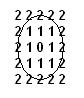
\includegraphics[scale=1]{distEuclidea.png} 
\end{center} 
 
D_{4} Distancia euclidea	D4(p, q) = |x-s| + |y-t|  	(Si D_{4}=1 \rightarrow 4-vecinos de p)
\begin{center}
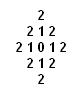
\includegraphics[scale=1]{distEuclidea4.png} 
\end{center} 
 
D_{8} Distancia de ajedrez	D8(p, q) = max(|x-s| , |y-t|) 		(Si D_{8}=1 \rightarrow 8-vecinos de p)
\begin{center}
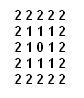
\includegraphics[scale=1]{distAjedrez.png} 
\end{center} 

Las t�cnicas mas utilizadas en el suavizado es el uso de m�scaras de convoluci�n (plantillas, ventanas o filtros). Normalmente son matrices 3x3, pero en nuestro caso hemos utilizado matrices 5x5.

\begin{center}
\begin{tabular}{|c|c|c|}
\hline w1(x-1, y-1) & w2(x, y-1) & w3(x+1, y-1) \\ 
\hline w4(x-1, y) & w5(x, y) & w6(x+1, y) \\ 
\hline w7(x-1, y+1) & w8(x, y+1) & w9(x+1, y+1) \\ 
\hline 
 Mascara 3x3
\end{tabular} 
\end{center} 

\section{Tipos}
Hay varios tipos de suavizado:
\begin{itemize}
\item Promedio del entorno de vecindad.
\item Filtrado de la mediana.
\item Promedio de la imagen.
\item Suavizado binario de im�genes.
\end{itemize} 

\section{Promedio del entorno de vecindad}
Es el m�todo que hemos utilizado en el preprocesamiento de las im�genes recibidas por la c�mara.
Se utiliza para la eliminaci�n de ruidos y otros efectos debidos a la cuantizaci�n o a perturbaciones. La raz�n de haber utilizado un suavizado al principio fue para crear un difuminado de la imagen y que futuros filtrados sean mas uniformes. Siempre el objetivo buscado es generar una imagen lo suficientemente simple y objetiva para ser entendida por la red neuronal.

Las desventajas de este m�todo son que desdibuja contornos y detalles de forma, pero en nuestro caso concreto esto no tiene relevancia.
\begin{center}
\textbf{g(x, y) = $ (\dfrac{1}{K}) * \Sigma f(n, m) $} 
\end{center} 
(sumatorio de 0 a K, siendo K el numero total de puntos de la vecindad)

M�todo:
\begin{center}
Se utiliza una m�scara de 5x5 \rightarrow  wi = 1/25
\end{center} 
	 
\begin{center}
\begin{tabular}{|c|c|}
\hline 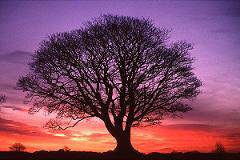
\includegraphics[scale=1]{arbol1.png}  & 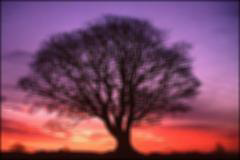
\includegraphics[scale=1]{arbolSuav.png}  \\ 
\hline 
\end{tabular} 
Dos representaciones de la misma imagen. La imagen de la izquierda es la imagen original y la de la derecha es la imagen despu�s de aplicarle el suavizado promedio del entorno de vecindad.
\end{center} 

